% =============================================================================
% TP 2.1 - Generadores Pseudoaleatorios
% Universidad Tecnológica Nacional – FRRO
% Materia: Simulación 2026
%
% Compilación (desde la carpeta tp2_1/informe/):
%   pdflatex main.tex
%   bibtex main
%   pdflatex main.tex
%   pdflatex main.tex
%
% En Overleaf: subir main.tex, referencias.bib y la carpeta graficos/.
% =============================================================================

\documentclass[a4paper, 11pt]{article}

% --- Codificación y lenguaje ---
\usepackage[utf8]{inputenc}
\usepackage[T1]{fontenc}
\usepackage[spanish, es-nodecimaldot]{babel}

% --- Matemática ---
\usepackage{amsmath}
\usepackage{amssymb}

% --- Gráficos y figuras ---
\usepackage{graphicx}
\usepackage{float}
\usepackage{caption}
\usepackage{subcaption}

% --- Tablas ---
\usepackage{booktabs}
\usepackage{array}
\usepackage{multirow}

% --- Formato ---
\usepackage[margin=2.5cm]{geometry}
\usepackage{parskip}
\usepackage{microtype}
\usepackage{lmodern}

% --- Hipervínculos ---
\usepackage[
  colorlinks=true,
  linkcolor=blue!70!black,
  citecolor=blue!70!black,
  urlcolor=blue!70!black
]{hyperref}

% --- Código fuente ---
\usepackage{listings}
\usepackage{xcolor}

\lstdefinestyle{python}{
  language=Python,
  basicstyle=\ttfamily\small,
  keywordstyle=\color{blue!80!black}\bfseries,
  commentstyle=\color{gray},
  stringstyle=\color{orange!80!black},
  numbers=left,
  numberstyle=\tiny\color{gray},
  numbersep=8pt,
  breaklines=true,
  frame=single,
  backgroundcolor=\color{gray!8},
  showstringspaces=false,
  tabsize=4,
  captionpos=b
}

% =============================================================================

\title{%
  \textbf{TP 2.1 -- Generadores de Números Pseudoaleatorios} \\[6pt]
  \large Universidad Tecnológica Nacional -- FRRO \\
  \large Materia: Simulación -- Año 2026
}

\author{
  Ceballos, R. \\
  \texttt{rceballos.work@gmail.com}
}

\date{1 de junio, 2026}

% =============================================================================

\begin{document}

\maketitle

% ---------------------------------------------------------------------------
\begin{abstract}
El presente trabajo describe la implementación y evaluación de tres generadores
de números pseudoaleatorios en Python~3: el Generador Congruencial Lineal (GCL),
el método de Cuadrados Medios de Von~Neumann y el Mersenne Twister de la
biblioteca estándar de Python. Cada generador fue evaluado con cuatro pruebas
estadísticas (Chi-cuadrado, Kolmogorov-Smirnov, Rachas y Poker) aplicadas sobre
$n = 10\,000$ muestras al nivel de significancia $\alpha = 0{,}05$. Los
resultados muestran que el GCL aprueba tres de las cuatro pruebas y presenta
una leve correlación detectada por el test de rachas; el método de Cuadrados
Medios degenera a cero en pocas iteraciones y falla todas las pruebas; el
Mersenne Twister aprueba la totalidad de las pruebas y se confirma como
referencia de calidad.
\end{abstract}

% ---------------------------------------------------------------------------
\section{Introducción}

Un número pseudoaleatorio es un número producido por un algoritmo determinista
que, sin embargo, exhibe propiedades estadísticas similares a las de una secuencia
verdaderamente aleatoria~\cite{knuth1997art}. La aparente aleatoriedad es la razón
por la que estos generadores resultan útiles en simulación computacional: a
igualdad de semilla inicial producen siempre la misma secuencia, lo que permite
la reproducibilidad de los experimentos.

Los generadores de números pseudoaleatorios (GNPA) son componentes fundamentales
en simulación de sistemas, métodos de Monte Carlo, criptografía y computación
científica. La calidad de un generador se mide a partir de propiedades como
uniformidad, independencia entre valores sucesivos, período largo y eficiencia
computacional~\cite{law2015simulation}.

En este trabajo se implementan y comparan tres generadores:
\begin{itemize}
  \item \textbf{GCL} (Generador Congruencial Lineal): el más utilizado
        históricamente, propuesto por Lehmer (1951) y analizado exhaustivamente
        por Knuth~\cite{knuth1997art}.
  \item \textbf{Cuadrados Medios}: introducido por Von~Neumann en 1946 como
        uno de los primeros GNPA computacionales~\cite{vonneumann1951various}.
  \item \textbf{Mersenne Twister}: implementado en el módulo \texttt{random}
        de Python, con período de $2^{19937}-1$~\cite{matsumoto1998mersenne}.
\end{itemize}


% ---------------------------------------------------------------------------
\section{Métodos}

\subsection{Generador Congruencial Lineal (GCL)}

El GCL genera una secuencia de enteros $\{X_n\}$ mediante la recurrencia:

\begin{equation}
  X_{n+1} = (a \cdot X_n + c) \bmod m
  \label{eq:gcl}
\end{equation}

donde $a$ es el multiplicador, $c$ el incremento, $m$ el módulo y $X_0$ la
semilla. El número pseudoaleatorio en $[0, 1)$ se obtiene como $U_n = X_n / m$.

Para garantizar período completo de longitud $m$ se deben cumplir las condiciones
del teorema de Hull-Dobell~\cite{knuth1997art}: $\text{mcd}(c, m) = 1$, todo factor
primo de $m$ divide a $a-1$, y si $4 \mid m$ entonces $4 \mid (a-1)$.

En este trabajo se utilizan los parámetros de Numerical Recipes~\cite{press1992numerical}:

\begin{equation}
  a = 1\,664\,525, \quad c = 1\,013\,904\,223, \quad m = 2^{32}
  \label{eq:gcl_params}
\end{equation}

que satisfacen las condiciones del teorema y producen un período máximo de
$m = 4\,294\,967\,296$.

\subsection{Generador de Cuadrados Medios}

El método de Cuadrados Medios, propuesto por Von~Neumann
\cite{vonneumann1951various}, opera sobre un número entero de $d$ dígitos.
Para obtener el siguiente valor se eleva al cuadrado el valor actual y se
extraen los $d$ dígitos centrales del resultado (que tiene $2d$ dígitos,
completado con ceros a la izquierda si fuera necesario):

\begin{equation}
  X_{n+1} = \left\lfloor \frac{X_n^2 \bmod 10^{\frac{3d}{2}}}{10^{\frac{d}{2}}} \right\rfloor
  \label{eq:cuad_medios}
\end{equation}

El número en $[0, 1)$ se obtiene como $U_n = X_n / 10^d$.

Este método tiene dos deficiencias conocidas: (a) período muy corto en la
mayoría de las semillas y (b) tendencia a colapsar en el valor cero, del que
no puede escapar dado que $0^2 = 0$~\cite{knuth1997art}. Se implementa con
$d = 4$ dígitos y semilla $X_0 = 3141$.

\subsection{Mersenne Twister}

El Mersenne Twister (MT19937), diseñado por Matsumoto y Nishimura
\cite{matsumoto1998mersenne}, es un GNPA basado en una recurrencia lineal
sobre $\text{GF}(2)$ (cuerpo de Galois de dos elementos). Sus características
principales son:

\begin{itemize}
  \item Período: $2^{19937} - 1 \approx 4{,}3 \times 10^{6001}$.
  \item Equidistribución en 623 dimensiones en punto fijo de 32 bits.
  \item Supera la mayoría de los tests estadísticos estándar.
\end{itemize}

Se utiliza a través del módulo \texttt{random} de Python con semilla fija
$s = 12345$ como referencia de calidad~\cite{python_random}.

\subsection{Tests estadísticos}

Se aplican cuatro tests al nivel de significancia $\alpha = 0{,}05$, sobre
$n = 10\,000$ muestras por generador. En todos los casos la hipótesis nula
$H_0$ es que los números provienen de una distribución uniforme $U(0,1)$
e independiente.

\subsubsection{Test Chi-cuadrado de uniformidad}

Se divide $[0, 1)$ en $k = 10$ intervalos iguales y se cuenta la frecuencia
observada $O_i$ en cada uno. La frecuencia esperada bajo $H_0$ es $E_i = n/k$.
El estadístico es:

\begin{equation}
  \chi^2 = \sum_{i=1}^{k} \frac{(O_i - E_i)^2}{E_i}
  \label{eq:chi2}
\end{equation}

con $k-1 = 9$ grados de libertad. Se rechaza $H_0$ si $\chi^2 > \chi^2_{9,\,0{,}95} = 16{,}919$.

\subsubsection{Test de Kolmogorov-Smirnov}

Se compara la función de distribución acumulada empírica $F_n(x)$ con la
teórica $F(x) = x$ (distribución uniforme). El estadístico es:

\begin{equation}
  D_n = \sup_{x} \left|F_n(x) - F(x)\right|
  \label{eq:ks}
\end{equation}

El valor crítico aproximado (Massey, 1951) para $\alpha = 0{,}05$ es:
\begin{equation}
  d_{crit} = \sqrt{\frac{-\ln(\alpha/2)}{2n}}
  \label{eq:ks_critico}
\end{equation}

Se rechaza $H_0$ si $D_n > d_{crit}$.

\subsubsection{Test de Rachas}

Una racha es una secuencia máxima de valores consecutivos todos por encima
o todos por debajo de la mediana muestral. Sea $n_1$ la cantidad de valores
por encima y $n_2 = n - n_1$ la cantidad por debajo, y $R$ el número de
rachas observadas. Bajo $H_0$:

\begin{equation}
  E[R] = \frac{2\,n_1\,n_2}{n} + 1, \qquad
  \text{Var}[R] = \frac{2\,n_1\,n_2\,(2\,n_1\,n_2 - n)}{n^2\,(n-1)}
  \label{eq:rachas}
\end{equation}

El estadístico de prueba es:
\begin{equation}
  Z = \frac{R - E[R]}{\sqrt{\text{Var}[R]}} \xrightarrow{d} \mathcal{N}(0,1)
  \label{eq:rachas_z}
\end{equation}

Es un test bilateral: se rechaza $H_0$ si $|Z| > z_{0{,}025} = 1{,}960$.

\subsubsection{Test de Poker}

Los números se agrupan en conjuntos de $d = 5$ elementos; cada elemento se
discretiza a uno de $m = 10$ posibles ``dígitos'' (tomando $\lfloor x \cdot 10 \rfloor$).
Se clasifica cada grupo según la cantidad $k$ de dígitos distintos que contiene.

La probabilidad teórica de obtener exactamente $k$ valores distintos en $d$
extracciones con reemplazo de $m$ posibles valores es~\cite{knuth1997art}:

\begin{equation}
  P(k) = \frac{\binom{m}{k} \cdot S(d,k) \cdot k!}{m^d}
  \label{eq:poker_prob}
\end{equation}

donde $S(d,k)$ es el número de Stirling del segundo tipo. Para $d=5$, $m=10$:

\begin{table}[H]
  \centering
  \caption{Probabilidades teóricas del test de Poker ($d=5$, $m=10$).}
  \label{tab:poker_probs}
  \begin{tabular}{cccc}
    \toprule
    $k$ & Descripción & $P(k)$ & $E$ (grupos = 2000) \\
    \midrule
    $\leq 2$ & Todos/casi iguales & $0{,}0136$ & $27{,}2$ \\
    $3$      & Tres distintos     & $0{,}1800$ & $360{,}0$ \\
    $4$      & Cuatro distintos   & $0{,}5040$ & $1008{,}0$ \\
    $5$      & Todos distintos    & $0{,}3024$ & $604{,}8$ \\
    \bottomrule
  \end{tabular}
\end{table}

Las categorías $k=1$ y $k=2$ se fusionan (frecuencia esperada $< 5$).
Se aplica un Chi-cuadrado sobre las 4 categorías resultantes con $4-1=3$
grados de libertad; se rechaza $H_0$ si $\chi^2 > \chi^2_{3,\,0{,}95} = 7{,}815$.

\subsection{Implementación}

El código está organizado en tres archivos dentro de \texttt{tp2\_1/}:

\begin{itemize}
  \item \texttt{generadores.py}: clases \texttt{GCL}, \texttt{CuadradosMedios}
        y \texttt{MersenneTwister}, cada una con un método \texttt{generar(n)}.
  \item \texttt{tests\_estadisticos.py}: funciones para los cuatro tests,
        retornando un objeto \texttt{ResultadoTest} con estadístico, valor
        crítico, p-valor y resultado (aprobado/rechazado).
  \item \texttt{main.py}: orquestación, generación de gráficos e impresión
        de la tabla resumen.
\end{itemize}

El fragmento central del GCL es:

\begin{lstlisting}[style=python, caption={Implementación del Generador Congruencial Lineal.}]
def generar(self, n: int) -> list[float]:
    numeros: list[float] = []
    x = self.semilla
    for _ in range(n):
        x = (self.a * x + self.c) % self.m
        numeros.append(x / self.m)
    return numeros
\end{lstlisting}

Y el del test Chi-cuadrado:

\begin{lstlisting}[style=python, caption={Test Chi-cuadrado de uniformidad.}]
def test_chi_cuadrado(numeros, k=10, alpha=0.05):
    n = len(numeros)
    esperado = n / k
    observado = [0] * k
    for x in numeros:
        idx = min(int(x * k), k - 1)
        observado[idx] += 1
    chi2 = sum((o - esperado)**2 / esperado for o in observado)
    # gl = k - 1 grados de libertad
    p_valor = 1 - chi2_dist.cdf(chi2, k - 1)
    return chi2, p_valor
\end{lstlisting}


% ---------------------------------------------------------------------------
\section{Resultados}

Se generaron $n = 10\,000$ números con cada generador (semilla $= 12345$ para
GCL y MT; semilla $= 3141$ para Cuadrados Medios) y se aplicaron los cuatro
tests estadísticos con $\alpha = 0{,}05$.

\subsection{Tabla comparativa de resultados}

\begin{table}[H]
  \centering
  \caption{Resultados de los cuatro tests estadísticos ($n = 10\,000$, $\alpha = 0{,}05$).
    Se indica el estadístico calculado, el valor crítico y el resultado.}
  \label{tab:resultados}
  \small
  \begin{tabular}{llcccc}
    \toprule
    \multirow{2}{*}{Generador} & \multirow{2}{*}{Test} &
      \multirow{2}{*}{Estadístico} & \multirow{2}{*}{Valor crítico} &
      \multirow{2}{*}{p-valor} & \multirow{2}{*}{Resultado} \\
    & & & & & \\
    \midrule
    \multirow{4}{*}{GCL}
      & Chi-cuadrado    & $14{,}160$ & $16{,}919$ & $0{,}117$ & \textbf{APROBADO} \\
      & K-S             & $0{,}006$  & $0{,}014$  & $0{,}867$ & \textbf{APROBADO} \\
      & Rachas          & $2{,}100$  & $1{,}960$  & $0{,}036$ & \textit{RECHAZADO} \\
      & Poker           & $1{,}011$  & $7{,}815$  & $0{,}799$ & \textbf{APROBADO} \\
    \midrule
    \multirow{4}{*}{Cuadrados Medios}
      & Chi-cuadrado    & $89900{,}03$ & $16{,}919$ & $\approx 0$ & \textit{RECHAZADO} \\
      & K-S             & $0{,}989$  & $0{,}014$  & $\approx 0$ & \textit{RECHAZADO} \\
      & Rachas          & $\infty$   & $1{,}960$  & $0{,}000$ & \textit{RECHAZADO} \\
      & Poker           & $144911{,}80$ & $7{,}815$ & $\approx 0$ & \textit{RECHAZADO} \\
    \midrule
    \multirow{4}{*}{Mersenne Twister}
      & Chi-cuadrado    & $5{,}884$  & $16{,}919$ & $0{,}752$ & \textbf{APROBADO} \\
      & K-S             & $0{,}008$  & $0{,}014$  & $0{,}586$ & \textbf{APROBADO} \\
      & Rachas          & $1{,}900$  & $1{,}960$  & $0{,}057$ & \textbf{APROBADO} \\
      & Poker           & $0{,}042$  & $7{,}815$  & $0{,}998$ & \textbf{APROBADO} \\
    \bottomrule
  \end{tabular}
\end{table}

\subsection{Distribución de los números generados}

La Figura~\ref{fig:histogramas} muestra los histogramas de los tres generadores.
El GCL y el Mersenne Twister presentan distribuciones aproximadamente uniformes;
el Cuadrados Medios exhibe una concentración casi total en el valor cero, indicando
degeneración temprana del generador.

\begin{figure}[H]
  \centering
  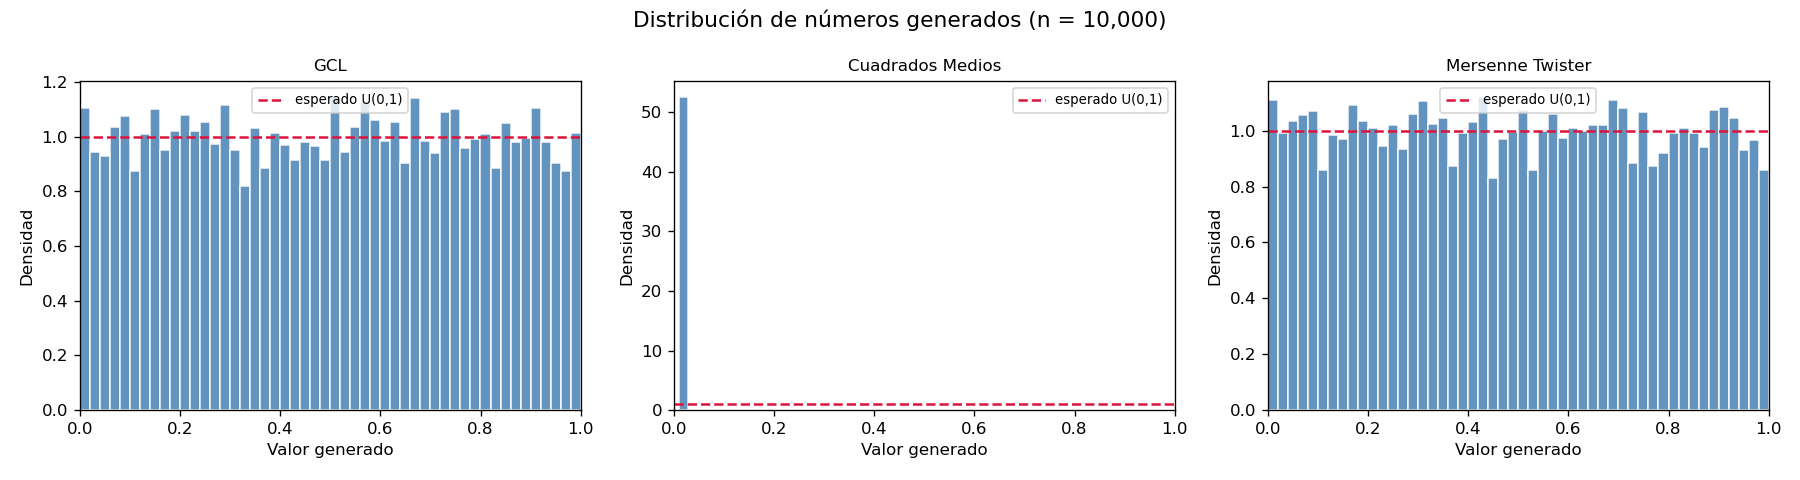
\includegraphics[width=\linewidth]{../graficos/histogramas.png}
  \caption{Histograma de distribución de los $10\,000$ números generados por
    cada generador. La línea roja discontinua indica la densidad esperada para
    $U(0,1)$.}
  \label{fig:histogramas}
\end{figure}

\subsection{Función de distribución acumulada}

La Figura~\ref{fig:cdf} compara la CDF empírica de cada generador con la CDF
teórica de la distribución $U(0,1)$ (línea $F(x) = x$). La distancia máxima
entre ambas curvas corresponde al estadístico $D_n$ del test de Kolmogorov-Smirnov.
Para el GCL y el Mersenne Twister, las curvas son prácticamente indistinguibles.
Para Cuadrados Medios, la CDF empírica presenta un salto abrupto cerca de $x=0$,
consistente con la degeneración del generador.

\begin{figure}[H]
  \centering
  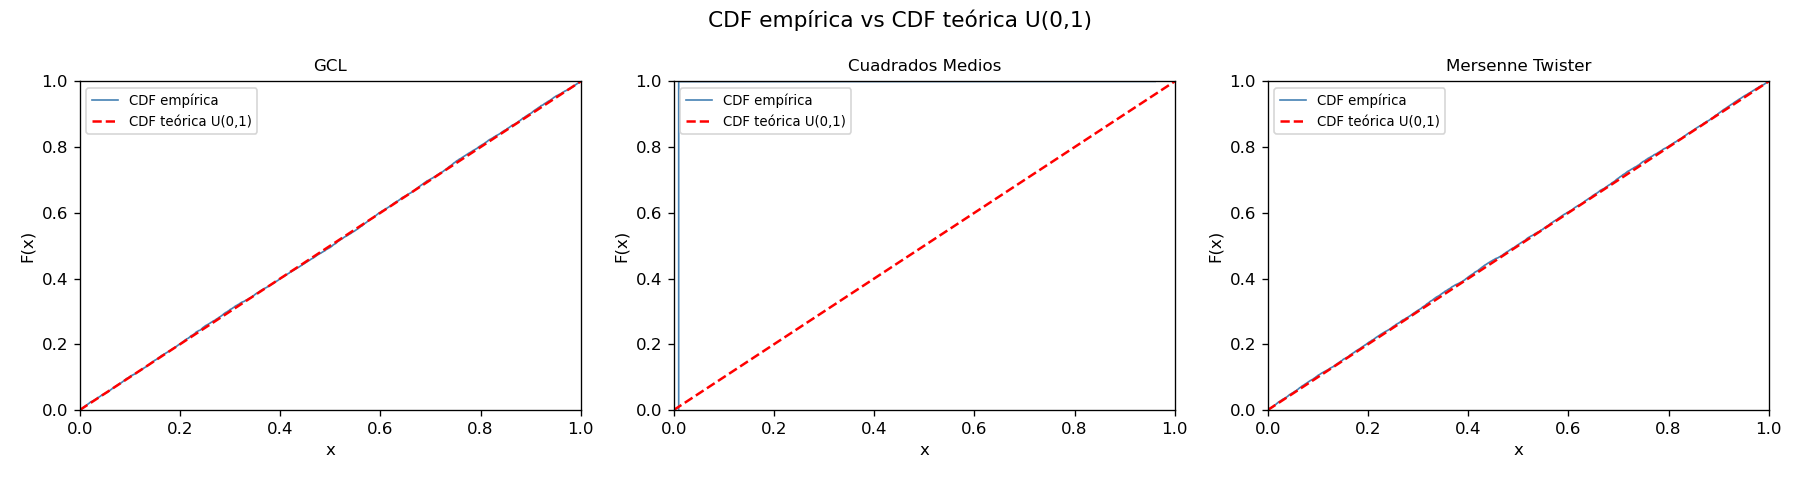
\includegraphics[width=\linewidth]{../graficos/cdf.png}
  \caption{CDF empírica (azul) vs. CDF teórica $U(0,1)$ (roja). Una CDF empírica
    que se superpone casi perfectamente a la línea $F(x) = x$ indica buena uniformidad.}
  \label{fig:cdf}
\end{figure}

\subsection{Diagrama de correlación serial}

La Figura~\ref{fig:correlacion} muestra el diagrama de dispersión de $x_n$ vs
$x_{n+1}$ para los primeros $2000$ pares de cada generador. Un generador con
buena independencia produce un nube de puntos uniforme sobre el cuadrado
$[0,1)^2$, sin patrones visibles. Los tres generadores exhiben el comportamiento
esperado salvo el Cuadrados Medios, donde todos los puntos colapsan al origen.

\begin{figure}[H]
  \centering
  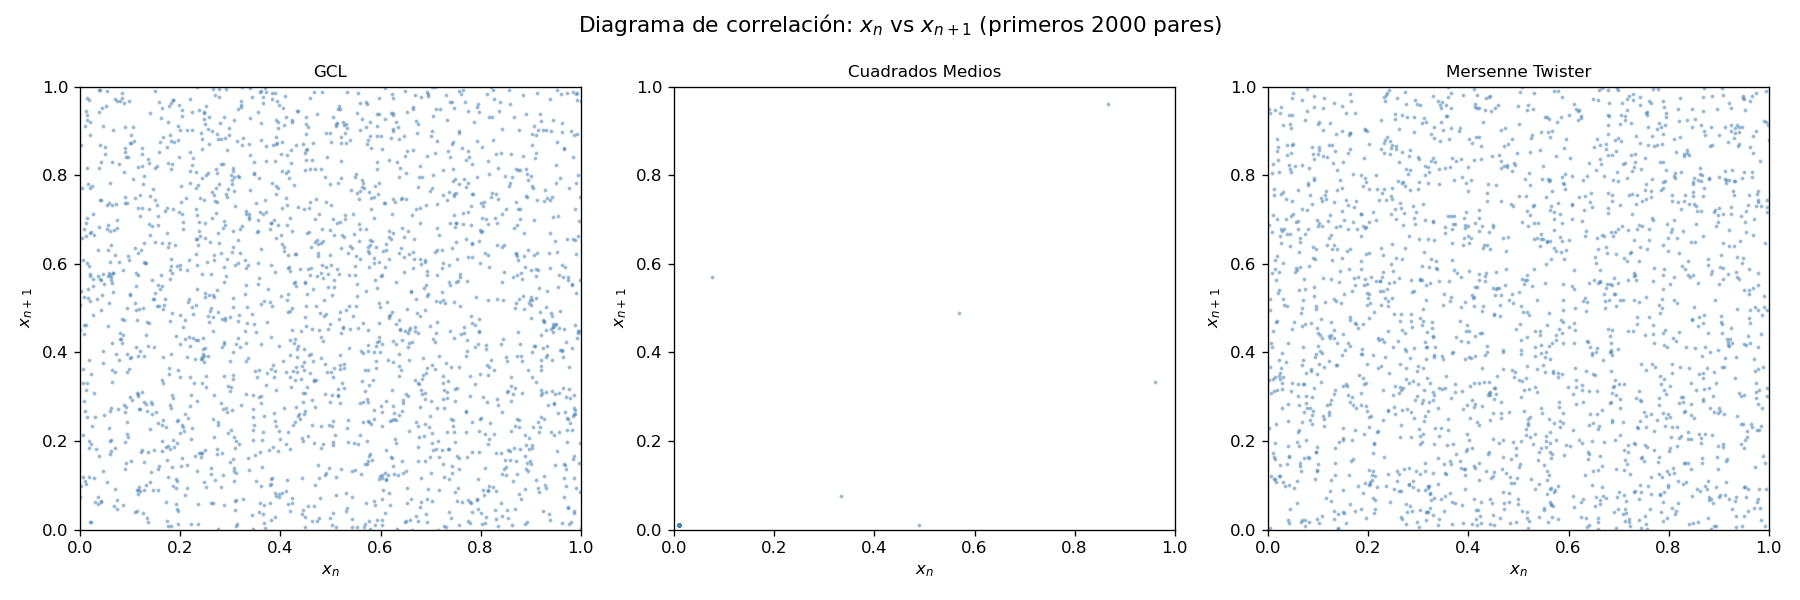
\includegraphics[width=\linewidth]{../graficos/correlacion.png}
  \caption{Diagrama de correlación serial ($x_n$ vs $x_{n+1}$, primeros $2000$ pares).
    Un patrón visible o una concentración de puntos indica dependencia entre valores
    sucesivos.}
  \label{fig:correlacion}
\end{figure}


% ---------------------------------------------------------------------------
\section{Discusión}

\subsection{GCL: comportamiento general}

El GCL con los parámetros de Numerical Recipes aprueba el test Chi-cuadrado
($\chi^2 = 14{,}160 < 16{,}919$, $p = 0{,}117$) y el test de Kolmogorov-Smirnov
($D_n = 0{,}006 \ll 0{,}014$, $p = 0{,}867$), lo que confirma que la
distribución empírica es consistente con $U(0,1)$. El test de Poker también
es superado ampliamente ($\chi^2 = 1{,}011$, $p = 0{,}799$).

Sin embargo, el test de Rachas resulta en $|Z| = 2{,}100 > 1{,}960$ ($p = 0{,}036$),
indicando una leve correlación entre valores sucesivos. Este resultado, aunque
marginalmente significativo, es característico de todos los GCL: la relación
lineal de la recurrencia (ec.~\ref{eq:gcl}) implica que pares consecutivos
$(X_n, X_{n+1})$ no cubren de forma completamente uniforme el cuadrado
$[0,m)^2$, un fenómeno conocido como \emph{estructura de hiperplanos}
\cite{knuth1997art}. L'Ecuyer~\cite{lecuyer1988efficient} recomienda combinar
dos o más GCL para mitigar este efecto.

El período máximo de $m = 2^{32} \approx 4{,}3 \times 10^9$ resulta adecuado
para aplicaciones de simulación moderadas, aunque insuficiente para simulaciones
de alta dimensión.

\subsection{Cuadrados Medios: degeneración}

El generador de Cuadrados Medios con semilla $X_0 = 3141$ y $d = 4$ dígitos
degenera al valor cero en pocas iteraciones: una vez que $X_n = 0$, el valor
$X_{n+1} = 0^2 = 0$ queda fijo para siempre. El estadístico Chi-cuadrado de
$89\,900{,}03$ (frente a un valor crítico de $16{,}919$) refleja que casi la
totalidad de los $10\,000$ valores cayeron en el primer intervalo $[0;\,0{,}1)$.
La distancia KS de $0{,}989$ confirma que la distribución empírica no tiene
ninguna similitud con $U(0,1)$.

Esta limitación es una característica estructural del método: el número de
estados posibles (secuencias distintas de $d$ dígitos) es finito, muchas
semillas llevan rápidamente a un ciclo de período 1 (el cero), y no existe
garantía de período largo para ninguna semilla. Von~Neumann ya era consciente
de esta debilidad al proponer el método \cite{vonneumann1951various}; hoy el
método de Cuadrados Medios tiene únicamente valor histórico y didáctico.

\subsection{Mersenne Twister: referencia de calidad}

El Mersenne Twister aprueba los cuatro tests con amplios márgenes:
p-valores de $0{,}752$ (Chi-cuadrado), $0{,}586$ (KS), $0{,}057$ (Rachas)
y $0{,}998$ (Poker). Su período astronómico ($2^{19937}-1$) y la propiedad de
equidistribución en 623 dimensiones lo hacen apto para prácticamente cualquier
simulación general~\cite{matsumoto1998mersenne}. Es el generador por defecto
de Python, R, MATLAB y la mayoría de los lenguajes de alto nivel modernos.

Nótese que el test de Rachas del MT da $|Z| = 1{,}900$, apenas por debajo del
umbral de $1{,}960$ ($p = 0{,}057 > 0{,}05$): un resultado muy cercano al límite
pero que no rechaza la hipótesis nula.

\subsection{Comparación resumida}

\begin{table}[H]
  \centering
  \caption{Resumen comparativo de los generadores evaluados.}
  \label{tab:comparacion}
  \begin{tabular}{lccc}
    \toprule
    Característica         & GCL      & Cuad. Medios & MT \\
    \midrule
    Período                & $2^{32}$ & $\leq 10^4$ (práct. $\ll$) & $2^{19937}-1$ \\
    Tests aprobados (de 4) & 3        & 0            & 4 \\
    Uniformidad            & Buena    & Nula         & Muy buena \\
    Independencia          & Parcial  & Nula         & Muy buena \\
    Complejidad impl.      & Baja     & Baja         & Alta \\
    Uso recomendado        & Simulac. básica & Solo didáctico & General \\
    \bottomrule
  \end{tabular}
\end{table}


% ---------------------------------------------------------------------------
\section{Conclusiones}

\begin{enumerate}
  \item El \textbf{Generador Congruencial Lineal} con los parámetros de
        Numerical Recipes produce secuencias con buena uniformidad (aprueba
        Chi-cuadrado y KS) y buena distribución de patrones (aprueba Poker).
        La detección de leve correlación serial por el test de Rachas
        ($|Z| = 2{,}10$, $p = 0{,}036$) es consistente con la conocida
        \textit{estructura de hiperplanos} de los GCL, pero no compromete su
        utilidad en simulaciones generales de escala moderada.

  \item El \textbf{método de Cuadrados Medios} es inadecuado para simulación:
        degenera al cero en pocas iteraciones con la semilla utilizada,
        produciendo secuencias completamente no uniformes e independientes.
        Su único valor es histórico y didáctico, ilustrando las dificultades
        de diseño de un GNPA robusto.

  \item El \textbf{Mersenne Twister} supera los cuatro tests estadísticos con
        amplios márgenes, confirmando su condición de generador de referencia.
        Para simulaciones generales donde se requiere buena calidad estadística
        y período muy largo, es la elección apropiada.

  \item La combinación de múltiples tests estadísticos es fundamental para
        evaluar un generador: ningún test por sí solo es suficiente. El GCL
        hubiera sido declarado apto con solo los tests de uniformidad (Chi-cuadrado
        y KS), pero el test de independencia (Rachas) revela una debilidad
        estructural que los tests de uniformidad no capturan.
\end{enumerate}

% ---------------------------------------------------------------------------
\bibliographystyle{unsrt}
\bibliography{referencias}

\end{document}
